\documentclass[a4paper,12pt]{report}

% font stuff
\usepackage{fouriernc}
\usepackage[T1]{fontenc}

\usepackage{amsmath}
\usepackage{amssymb}
\usepackage{amsthm}
\usepackage[retainorgcmds]{IEEEtrantools}
\usepackage{enumitem} % no space between enum lists

\usepackage{tikz}
\usetikzlibrary{positioning}
\usetikzlibrary{matrix}


\newcommand{\below}{\sqsubseteq}
\newcommand{\arr}{\rightarrow}
\newcommand{\Arr}{\Rightarrow}
\newcommand{\todo}[1]{\smallskip \noindent \emph{todo: #1} \smallskip}
%\newcommand{\todo}[1]{}
\newcommand{\semantics}[1]{\llbracket #1 \rrbracket}
\newcommand{\lub}{\bigsqcup}
\newcommand{\set}[1]{\{\,#1\,\}}
% partial function arrow
% https://tex.stackexchange.com/questions/47142/how-to-tex-an-arrow-with-vertical-stroke
\newcommand{\pfun}{\mathrel{\ooalign{\hfil$\mapstochar\mkern5mu$\hfil\cr$\to$\cr}}}
\newcommand{\isdefined}{\!\downarrow}
\newcommand{\Cppo}{\text{Cppo}}

\newcommand{\bbN}{\mathbb{N}}
\newcommand{\bbC}{\mathbb{C}}
\newcommand{\bbD}{\mathbb{D}}
\newcommand{\bbE}{\mathbb{E}}

\newcommand{\aand}{\ \wedge \ }
\newcommand{\oor}{\ \vee \ }

\newcommand{\product}{\!\times\!}


% They all use the same counter, reset at section boundaries
% This gives a running number:
% Section 1
%   Theorem 1.1
%   Definition 1.2
%   Lemma 1.3
% Section 2
%   Definition 2.1
%   Lemma 2.2
%   ...
\newtheorem{definition}{Definition}[section]
\newtheorem{theorem}[definition]{Theorem}
\newtheorem{proposition}[definition]{Proposition}
\newtheorem{lemma}[definition]{Lemma}
\newtheorem{corollary}[definition]{Corollary}

\begin{document}

%\title{Domains for Algebraic Datatypes with Computation Steps}
%\author{Markus Klinik}
%\maketitle

\thispagestyle{empty}


\begin{center}

\textbf{\Large Domains for Algebraic Datatypes with Computation Steps}

\setlength{\baselineskip}{1.8\baselineskip}

\vspace{1.0cm}

by \\
Markus Klinik

\vspace{\fill}

\vspace{\fill}

A thesis submitted \\
in partial fulfillment of the \\
requirements for the degree of \\
Master of Mathematical Foundations of Computing Science \\

\vspace{\fill}

Faculty of Science \\
Radboud University Nijmegen

\vspace{\fill}

Supervised by \\
Herman Geuvers

\vspace{\fill}

August 2014 \\

\vspace{\fill}


\end{center}

\newpage

\addcontentsline{toc}{chapter}{Abstract}
\begin{center}
\textbf{\large Abstract}
\end{center}


Capretta \cite{Capretta2002} shows how to represent general recursion in a
type theory by using the datatype of coinductive natural numbers. We study the
denotational side by analyzing the relation between the domains of the lazy and
the coinductive natural numbers.  In particular we show that there exists a
mediating em\-bed\-ding projection pair between the final coalgebras of the
functors $1+X$ and $1+X+X$ in the category of complete pointed partial orders.
The construction is then generalized to show that arbitrary polynomial functors
can be augmented with computation steps in a similar way.


\newpage

\addcontentsline{toc}{chapter}{Acknowledgments}
\begin{center}
\textbf{\large Acknowledgments}
\end{center}

Two years ago, I left the comfortable environment of my friends, my family and
my coworkers to become a student, with the goal to look behind the scenes
of what I was doing in my day-to-day work as a software developer.

I would like to thank my friend Terry Stroup, who once gave, and still gives,
nourishment to my sparking interest in computer science, mathematics, and
philosophy. Without your encouragement, I would never have done this step.

I would also like to thank Tessa, Joshua and Kelley who made me feel welcome in
the Netherlands. I hope you all enjoyed our evenings together of cooking and
going out as much as I did.

Furthermore, many thanks to my supervisor Herman Geuvers, who took lots of
time and always had an open door to support me during the years of my study and
the time of my thesis.

Many people at Radboud University helped me solving small and big problems of
all sorts. In no particular order, thank you Rinus Plasmeijer, Helle Hansen, Wim
Veldman, Freek Wiedijk, Bas Westerbaan and Alexandra Silva.

Special thanks goes to my parents Josef and Veronika, who always unconditionally
supported all my decisions.



\newpage

\tableofcontents

\newpage

\listoffigures

\newpage

\chapter{Introduction}

Many type theories are strongly normalizing, but recursive functions may
diverge.  As a result, not all recursive functions are representable in such
theories. In his PhD thesis, Venanzio Capretta \cite{Capretta2002} shows how by
using a datatype that allows infinite elements, it is possible to represent
recursive functions as elements of a certain function type in his type theory.
He extends the formal system with the datatype of \emph{coinductive natural
numbers}, the greatest fixpoint of the functor $F(X) = 1 + X + X$.

We loosely take up this idea and study the denotational semantics of this
datatype. Dana Scott, one of the pioneers of programming language semantics,
discovered that complete partial orders and continuous functions lend themselves
well for giving denotations to programs. Our study takes place in this setting.

In this thesis we give an introduction to domain theory, and explain how it can
be used to guarantee the existence of denotations of certain recursive
specifications. We show how the functor $1+X+X$ arises as denotation of an
algebraic data type, and study from a computational viewpoint how it relates to
the lazy natural numbers. The method is then generalized to add computation
steps to arbitrary polynomial functors.

\section{Background}

Writing computer programs is a two-fold activity, as is proving mathematical
propositions. There is the syntactical exercise of producing well-formed
formulas, or programs, on the one hand, and mental manipulation of
abstract objects on the other. The idea is that formulas describe objects
and their properties in some semantic domain, often a mathematical set or
algebraic structure. In mathematics, the study of the relationship between
syntax and semantics is called model theory.  Classic model theory in particular
deals with first order predicate logic on the syntactic side and Tarski's notion
of model and truth on the semantic side.

One may wonder whether first order predicate logic is \emph{the} language for
mathematics. Is Tarski's definition of truth the \emph{true} one?  Are the
universal and existential quantifiers canonical? Why these two, why the
sentential connectives \emph{and} and \emph{or}? Similarly, for programming
languages we wonder which basic building blocks are essential for computation
and which other features can be expressed in terms of them.

Answers to such questions are often motivated not only by fundamental but also
practical considerations. It doesn't need much for a programming language to be
Turing complete, but that doesn't imply that it is convenient to write
algorithms in it. The prevalence of first order logic as the language of
mathematics comes for a big part from its usefulness for mathematicians to
convince others of their work. Similarly, domain theory turns out to be useful
for the study of programming language semantics.

\chapter{Domain Theory}

\section{Principles}

Programming languages usually feature some built-in basic objects like integers
and booleans. On a semantic level, we imagine programs as manipulations of such
objects, in particular we want to view algorithms as mathematical functions.
When studying the semantics of languages with higher-order functions,
which we think of as sugar coated untyped lambda calculi, where terms denote
both elements of and functions between some semantic domain $D$, we soon run
into the equation $D \cong D \arr D$ or variants thereof. The question
arises whether there is some $D$ satisfying this equation.

The untyped lambda calculus has fixpoint combinators. A semantics for the
untyped lambda calculus must reflect this, which means that if we want functions
of some kind as denotations for abstractions, such functions must have
fixpoints.

Furthermore, in most languages we can specify functions recursively. In such a
specification the name of the function being defined occurs both on the left and
right hand side of an equation, and the question arises whether such functions
are actually well-defined.

Domain theory offers tools to approach answers to such questions.

\begin{definition}

Let $D$ be a poset, $S \subseteq D$. The \emph{least upper bound} (``lub'') of
$S$ is an element $x \in D$ such that:

\begin{equation} \label{eqnLub1}
\forall y \in S \ldotp y \below x
\end{equation}
\begin{equation} \label{eqnLub2}
\forall z \in D \ldotp (\forall y \in S \ldotp y \below z) \implies x \below z
\end{equation}

The lub of S, if it exists, is denoted interchangeably by
\begin{IEEEeqnarray*}{rCl}
\lub S = \lub_{x \in S} x = \lub \set{x \mid x \in S}
\end{IEEEeqnarray*}

\end{definition}


Line (\ref{eqnLub1}) states that the lub is above all elements: it is an upper
bound, and (\ref{eqnLub2}) states that the lub is below any other upper bound:
it is the least such. If a lub exists, it is unique. It is therefore justified
to call it \emph{the} lub.


\begin{definition}

A \emph{chain} $C$ in a poset is a linearly ordered subset, that is
$\forall x,y \in C \ldotp x \below y \oor y \below x$

\end{definition}


\begin{definition}

Let $P$ be a poset. A set $D \subseteq P$ is \emph{directed} iff every finite
$F \subseteq D$ has an upper bound in $D$.

\end{definition}

Note that chains can be empty, while directed sets D can not, as the upper bound
of the empty set must be in D.

In literature on domain theory and semantics of programming languages, one
encounters three different definitions of complete partial orders.  There is
chain-completeness \cite{Moschovakis1994}, directed-completeness
\cite{DaveyPriestly1990}, \cite{Gunter1992}, and $\omega$-sequence-completeness
\cite{Allison1986}, \cite{Winskel1993}, \cite{BarrWells1990}. Abramsky and Jung
\cite{Abramsky1994} have a short discussion on the equivalence of these
definitions, but refer to further literature for proofs. The proof given here
occurs as an exercise in Davey and Priestly \cite{DaveyPriestly1990}.


\begin{definition} \label{defCpoDirectedComplete}

A directed-complete partial order, \emph{dcpo}, is a partial order where every
directed set has a least upper bound.

\end{definition}


\begin{definition} \label{defCpoChainComplete}

A chain-complete partial order, \emph{ccpo}, is a partial order where every
non-empty chain has a least upper bound.

\end{definition}


\begin{definition} \label{defCpoOmegaSequenceComplete}

An $\omega$-sequence-complete partial order, \emph{$\omega$-cpo}, is a partial
order where every non-decreasing sequence of elements $x_0 \below x_1 \below x_2
\below \ldots $ has a least upper bound.

\end{definition}


\begin{proposition} \label{propDefinitionsAreEquivalent}

These three definitions are equivalent.

\end{proposition}

For proposition \ref{propDefinitionsAreEquivalent} we give a round-robin proof,
of which two implications are fairly simple. The third implication is a bit more
involved, and requires the axiom of choice. We give a proof for the countable
case here because it is illustrative and it is the case we're interested in, and
refer to \cite{Markowsky1976} for the general case.


\begin{proof}

$\ref{defCpoDirectedComplete} \implies \ref{defCpoChainComplete}$: Every
non-empty chain is a directed set.

$\ref{defCpoChainComplete} \implies \ref{defCpoOmegaSequenceComplete}$:
The image of a non-decreasing $\omega$-sequence is a chain.

$\ref{defCpoOmegaSequenceComplete} \implies \ref{defCpoDirectedComplete}$: Let
$D$ be an $\omega$-cpo as in definition
\ref{defCpoOmegaSequenceComplete}, let $S = \set{x_0, x_1, x_2, \ldots}
\subseteq D$ be countable and directed. For each finite $F \subseteq S$, let
$u(F)$ be an upper bound of $F$ in $S$.  Construct a sequence of sets $P_n
\subseteq S$ as follows,
\begin{IEEEeqnarray*}{rCl}
P_0 & = & \set{x_0} \\
P_{n+1} & = & P_n \cup \set{u(P_n \cup y_n), y_n}
\end{IEEEeqnarray*}

where $y_n$ is the $x_i \in S\backslash P_n$ with the smallest possible $i$.

Every $P_n$ is directed: $P_0$ certainly is, and any finite subset of $P_{n+1}$
has $u(P_n \cup y_n) \in P_{n+1}$ as upper bound.  As every $P_n$ is finite and
directed, taking its lub is justified.

Consider the $\omega$-sequence $Q$ = $\set{\lub P_n}_{n \in \bbN}$. For
all $n$, we have $P_n \subseteq P_{n+1}$ and thus $\lub P_n \below \lub
P_{n+1}$, so $Q$ is non-decreasing, and therefore has a lub $z$.  Each $x \in S$
eventually occurs in some $P_n$, and we have $x \below \lub P_n \below z$, so
$z$ is an upper bound of $S$. Any upper bound $z'$ of $S$ is also an upper bound
of $Q$, and therefore $z \below z'$, i.e. $z$ is the lub of $S$.
\end{proof}


The complication in the third implication comes from the fact that a directed
set doesn't need to be linearly ordered. Every directed set does however contain
a chain which threads through the whole set, eventually rising above all
elements. The lub of the chain is then the lub of the directed set.

The equivalence between the three definitions justifies simply talking about
\emph{complete partial orders}, or \emph{cpos}. We use the definitions
interchangeably, which\-ev\-er is most handy in a given situation.

The fixpoint theorem constructs least fixpoints using countable chains.
Even if a domain is uncountable, the chains for which we want lubs are therefore
at most countable. Whenever we consider chains, we mean non-empty countable ones.

A non-empty countable chain $\set{x_n \mid x \in \bbN}$ is always also a non-decreasing
sequence \begin{IEEEeqnarray*}{c} x_0 \below x_1 \below x_2 \below \ldots
\end{IEEEeqnarray*} and vice versa.

A sequence is \emph{eventually constant} iff there exists an $n \in \bbN$ such
that for all $m > n$, $x_n = x_m$.  An eventually constant non-decreasing
sequence is equivalent to a finite chain, and vice versa.

\section{The Category Cppo}


\begin{definition}

A cpo $D$ is \emph{pointed} iff it has a bottom element $\bot$ which satisfies
$\forall d \in D \ldotp \bot \below d$. Such a pointed cpo is called
\emph{cppo}.

\end{definition}

\begin{definition}

Let $C$, $D$ be partial orders. A function $f : C \arr D$ is \emph{monotone} iff
it is order preserving, that is for all $x, y \in C$,
\begin{IEEEeqnarray*}{rCl}
  x \below y \implies f(x) \below f(y)
\end{IEEEeqnarray*}

\end{definition}

\begin{definition}

Let $C$, $D$ be cpos. A function $f : C \arr D$ is \emph{Scott-continuous} iff
it is monotone and preserves lubs, that is for all chains $P \subseteq C$,
\begin{IEEEeqnarray*}{rCl}
  f(\lub_{x \in P} x) = \lub_{x \in P} f(x)
\end{IEEEeqnarray*}

\end{definition}

Note that if a function preserves lubs, it is monotone,
\begin{IEEEeqnarray*}{rCl}
  x \below y \implies
  y = \lub \set{x, y} \implies
  f(y) = f(\lub \set{x, y}) = \lub \set{f(x), f(y)} \implies
  f(x) \below f(y)
\end{IEEEeqnarray*}
but in a proof of continuity of a function $f$ we usually need to prove
monotonicity as a first step so that for a chain $P$, $\set{f(x) \mid x \in P}$
is again a chain. This motivates the explicit mention of
monotonicity in the definition of Scott-continuity. Because we are only
concerned with this one notion of continuity here, we will call them simply
continuous functions.


\begin{lemma}

The identity function is continuous.

\end{lemma}

\begin{proof}
Let $P \in C$ be a chain. Then
\begin{IEEEeqnarray*}{c+x*}
id(\lub P) = \lub P = \lub_{x \in P} id(x) & \qedhere
\end{IEEEeqnarray*}
\end{proof}


\begin{lemma}

Composition of two continuous functions is continuous.

\end{lemma}

\begin{proof}
Let $f : C \arr D$, $g : D \arr E$ be continuous. Let $P \subseteq C$ be a
chain. Then
\begin{IEEEeqnarray*}{rCl+x*}
(g \circ f)(\lub P) & = & g(f(\lub_{x \in P} x)) \\
  & = & g( \lub_{x \in P} f(x) ) \\
  & = & \lub_{x \in P} g(f(x)) \\
  & = & \lub_{x \in P} (g \circ f)(x) & \qedhere
\end{IEEEeqnarray*}
\end{proof}


\begin{corollary}

The complete pointed posets, together with continuous functions between them form
a category.  This category is called Cppo.

\end{corollary}


\begin{definition}

A category with initial object has the \emph{fixpoint property} iff for all objects $A$ and arrows
$f : A \arr A$ there exists an arrow $Y(f) : 1 \arr A$, the fixpoint of f, such
that $Y(f) = f \circ Y(f)$.

\begin{center}
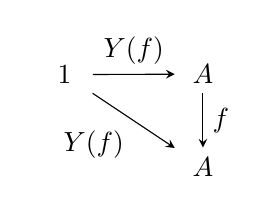
\begin{tikzpicture}
\matrix (m) [matrix of math nodes,row sep=2em,column sep=3em,minimum width=2em]
  {
     1 & A \\
     {} & A \\
  };
  \path[-stealth] (m-1-1) edge node [above] {$Y(f)$} (m-1-2);
  \path[-stealth] (m-1-1) edge node [below left] {$Y(f)$} (m-2-2);
  \path[-stealth] (m-1-2) edge node [right] {$f$} (m-2-2);
\end{tikzpicture}
\end{center}

\end{definition}


\begin{theorem} \label{thmFixpoint}

(Fixpoint Theorem) Cppo has the fixpoint property. In fact, every continuous
function on a cppo has a unique least fixpoint.

\end{theorem}

\begin{proof}

Let $D$ be a cppo, $f : D \arr D$ a continuous function. We have to show that
there exists an element $x \in D$ such that $x = f(x)$. Consider the set
\begin{equation*}
F = \set{f^n(\bot) \mid n \in \bbN}.
\end{equation*}
F is a chain: For $n = 0$
we have $f^0(\bot) = \bot \below f(\bot)$. Now assume that $f^n(\bot) \below
f^{n+1}(\bot)$. Then $f(f^n(\bot)) \below f(f^{n+1}(\bot))$, so $f^{n+1}(\bot)
\below f^{n+2}(\bot)$. Because $F$ is a chain and $D$ a cppo, $F$ has a lub $x =
\lub F$.  We calculate:
\begin{IEEEeqnarray*}{rCl}
f(x) & = & f(\lub F) \\
     & = & \lub f(F) \IEEEyesnumber \label{lineFContinuous} \\
     & = & \lub \set{ f(f^n(\bot)) \mid n \in \bbN } \\
     & = & \lub \set{ f^{n+1}(\bot) \mid n \in \bbN } \\
     & = & \lub \set{ f^n(\bot) \mid n \in \bbN }
           \IEEEyesnumber \label{lineLubLeastElement} \\
     & = & \lub F = x
\end{IEEEeqnarray*}
Line (\ref{lineFContinuous}) is because $f$ is continuous, and line
(\ref{lineLubLeastElement}) is because omitting the least element in a chain
doesn't affect the lub.

To see that $x$ is the least fixpoint, let $y = f(y)$ be a fixpoint of $f$. We
have:
\begin{IEEEeqnarray*}{rCl+x*}
\bot \below y & \implies & f(\bot) \below f(y) = y \\
 & \implies & \forall n \in \bbN \ldotp f^n(\bot) \below y \\
 & \implies & y \text{ is an upper bound of F} \\
 & \implies & \lub F = x \below y & \qedhere
\end{IEEEeqnarray*}
\end{proof}

This is the well-known fixpoint theorem, which is sometimes attributed to
Tarski, sometimes to Kleene, but while they both knew the result, its actual
origin seems to be lost in time \cite{Lassez1982}. The formulation given here
is due to Huwig \cite{Huwig1990}.


\begin{lemma} \label{lemCppoTerminalObject}
Cppo has a terminal object, the singleton $\set{\bot}$. \qed
\end{lemma}

\begin{lemma} \label{lemCppoBinaryProducts}
Cppo has binary products, defined pointwise. \qed
\end{lemma}

\begin{definition}
For $f, g : D \arr E$ continuous functions between domains, define $f \below g$ iff
$\forall d \in D \ldotp f(d) \below g(d)$.
\end{definition}

\begin{lemma} (Lubs of function chains are defined pointwise)
If $F$ is a chain of continuous
functions $D \arr E$ then the function
\begin{IEEEeqnarray*}{c}
d \mapsto \lub \set{f(d) \mid f \in F}
\end{IEEEeqnarray*}
is continuous and the least upper bound of $F$. \qed
\end{lemma}

\begin{lemma} \label{lemCppoExponentials}
Cppo has exponentials, that is
\begin{enumerate}[noitemsep]
  \item If $C$ and $D$ are cppos, then the space of continuous functions from
  $C$ to $D$, denoted $[C \arr D]$, forms a cppo.
  \item Currying and uncurrying are defined and are each others inverses. \qed
\end{enumerate}
\end{lemma}

\begin{corollary}
Cppo is cartesian closed.
\end{corollary}

A historical note on \ref{lemCppoExponentials}. Readers unfamiliar with domain
theory might be surprised that there exist domains $D$ which contain their own
function space $[D \arr D]$.  This result is due to Scott \cite{Scott1990}, who
\emph{"spent more days than [he cares] to remember trying to find one"}
\cite{Scott1993}. Intuitively, it is possible because the
requirement for functions in $[D \arr D]$ to be continuous restricts the
function space sufficiently as to not increase in cardinality.

So far, the situation in Cppo is quite satisfying. For a programming language
semantics however, we also want coproducts. Unfortunately, CCCs with fixpoints
cannot have coproducts, so the best we can hope for are approximations.  These
results were known before, but made precise by Huwig \cite{Huwig1990}.

\begin{definition}
A category is \emph{trivial} iff it has, up to isomorphism, exactly one object
with only the identity arrow.
\end{definition}

\begin{proposition} \label{propCCCNoFixpointCoproducts}
Any CCC with the fixpoint property and binary coproducts is trivial.
\end{proposition}

The proof uses some intermediary constructions which we introduce first.

\begin{definition}
An \emph{initial object} in a category is an object $0$ such that for any object
A there exists a unique arrow $0_A : 0 \arr A$.
\end{definition}

The prototypical example for an initial object is the empty set in Set. But
there are categories where initial objects behave differently than the empty set
in Set, perhaps unintuitively so. Important examples are categories where
objects are algebraic structures whose signature requires the existence of
elements, like monoids and groups. The initial objects in such categories are
not empty sets. In such categories the equivalence $0 \cong 0 \product A$ might
not hold.

\begin{lemma} \label{lem0xAisInitial}
In a CCC with initial object $0$ we have, for any object $A$, $0 \cong 0
\product A$.
\end{lemma}

\begin{proof}
It suffices to show that $0 \product A$ is initial. We know that the functor
$- \product A$ is left adjoint to the exponent functor $A \Arr -$, and
left adjoints preserve colimits (\cite{MacLane71}, IV.6, V.5). The initial object is the colimit of the
empty diagram. Therefore, $0 \product A$ is initial as well.
\end{proof}

As concise as abstract proofs like this become, they aren't very illustrative.
The following alternative proof of lemma \ref{lem0xAisInitial} is a bit longer,
but more insightful. The idea is that $0\product A$ must be initial because all
arrows $0 \product A \arr B$ are identical, and that is because their curried
counterparts are identical.

\begin{proof}
We show that $0 \product A$ is initial. Let $B$ be an object. Then the
arrow $f = 0_B \circ \pi_1\ :\ 0 \product A \arr B$ exists. To see that it is
unique, let $g : 0 \product A \arr B$ be an arrow. The exponent diagram of the
CCC gives rise to figure \ref{fig0xAInitialInCCCs},
\begin{figure}[ht]
\begin{center}
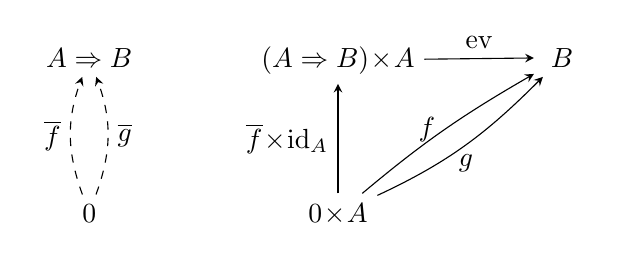
\begin{tikzpicture}
\matrix (m) [matrix of math nodes,row sep=4em,column sep=4em,minimum width=2em]
  {
     A \Arr B & (A \Arr B) \product A & B \\
     0 & 0 \product A \\
  };
  \path[-stealth, dashed] (m-2-1) [out=110,in=250] edge node [left] {$\overline{f}$} (m-1-1);
  \path[-stealth, dashed] (m-2-1) [out=70,in=290] edge node [right] {$\overline{g}$} (m-1-1);
  \path[-stealth] (m-1-2) edge node [above] {$\text{ev}$} (m-1-3)
    (m-2-2) edge node [left] {$\overline{f} \product \text{id}_A$} (m-1-2)
    (m-2-2) [out=40,in=210] edge node [left] {$f$} (m-1-3)
    (m-2-2) [out=25,in=225] edge node [below] {$g$} (m-1-3);
\end{tikzpicture}
\end{center}
\caption{$0\product A$ is initial in CCCs}
\label{fig0xAInitialInCCCs}
\end{figure}
where $\overline{f}$ is the curried counterpart of $f$. We have: $\overline{f} =
\overline{g}$, because $0$ is initial. Therefore $\overline{f}\product
\text{id}_A = \overline{g}\product \text{id}_A$, and
thus
\begin{IEEEeqnarray*}{c+x*}
f\ =\ \text{ev} \circ \overline{f}\product\text{id}_A
 \ =\ \text{ev} \circ \overline{g}\product\text{id}_A
 \ =\ g & \qedhere
\end{IEEEeqnarray*}
\end{proof}

\begin{lemma} \label{lem0isomorphic1}
In a category with fixpoints, initial and terminal objects are isomorphic.
\end{lemma}

\begin{proof}
As all endomorphisms have fixpoints, the identity on $0$ has a fixpoint
$Y(\text{id}_0) : 1 \arr 0$.  Composing it with the terminal map $!_0 : 0 \arr
1$ in both ways, the universal mapping properties of $0$ and $1$ give the
isomorphism $0 \cong 1$.
\end{proof}

\begin{proposition} \label{propCCCNoFixpointInitialObject}
Any CCC with the fixpoint property and initial object is trivial.
\end{proposition}

\begin{proof}
Let $A$ be an object.  Then $1 \cong 0 \cong 0 \product A \cong 1 \product A
\cong A$. The first two equivalences are lemmas \ref{lem0xAisInitial} and
\ref{lem0isomorphic1}, the second holds because $- \product A$ is a functor, and
the last one always holds.
\end{proof}

\newcommand{\true}{\text{tt}}
\newcommand{\false}{\text{ff}}

\begin{definition}
A \emph{Boolean algebra} is an algebraic structure $(A, \wedge, \vee, \neg,
\true, \false)$ where $\wedge, \vee$ are binary operations, $\neg$ is a unary
operation, and $\true, \false$ are distinguished elements of $A$, such that the
Boolean algebra axioms hold.
\end{definition}

The definition of Boolean algebra can be lifted to category theory in a
straightforward way. This enables us to lift theorems about Boolean algebras to
category theory. Operations and elements become arrows, and the Boolean algebra
axioms, which are all equations, become commutative diagrams:

\begin{definition}
A \emph{Boolean algebra object} in a category is an object A,
together with arrows $\wedge, \vee : A \product A \arr A$, $\neg : A \arr A$,
$\true, \false : 1 \arr A$ such that the diagrams corresponding to the boolean
algebra axioms commute.
\end{definition}

For example, the axiom $\forall p . p \wedge \true = p$ corresponds to the
requirement that the following diagram commutes.

\begin{figure}[h]
\begin{center}
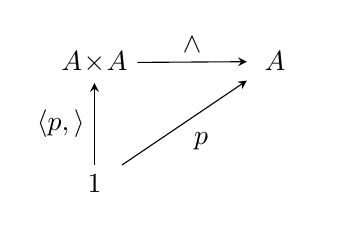
\begin{tikzpicture}
\matrix (m) [matrix of math nodes,row sep=3em,column sep=4em,minimum width=2em]
  {
     A \product A & A \\
     1 \\
  };
  \path[-stealth]
    (m-2-1) edge node [left] {$\langle p, \true \rangle$} (m-1-1)
    (m-1-1) edge node [above] {$\wedge$} (m-1-2)
    (m-2-1) edge node [below right] {$p$} (m-1-2) ;
\end{tikzpicture}
\end{center}
\end{figure}

\begin{lemma}
In a CCC with coproducts, $2 = 1+1$ is a boolean algebra object. \qed
\end{lemma}

\begin{lemma}
In a Boolean algebra $A$ where $\neg$ has a fixpoint $Y(\neg) = \neg Y(\neg)$,
all elements are identified.
\end{lemma}

\begin{proof}
\begin{IEEEeqnarray*}{rCl}
\true & = & Y(\neg) \oor \neg Y(\neg) \\
      & = & Y(\neg) \oor Y(\neg) \\
      & = & Y(\neg) \\
      & = & Y(\neg) \aand Y(\neg) \\
      & = & Y(\neg) \aand \neg Y(\neg) \\
      & = & \false
\end{IEEEeqnarray*}
Further, for any $a \in A$, $\false = a \wedge \false = a \wedge \true = a$.
\end{proof}

\begin{corollary}
\label{lemCoproductInjectionsIdentified}
In a CCC with fixpoints where the coproduct $1+1$ exists, the coproduct
injections $\true, \false : 1 \arr 1+1$ are identified. \qed
\end{corollary}

\begin{proposition}
\label{propCCCWith11IsTrivial}
Every CCC with fixpoints where the coproduct $1+1$ exists is trivial.
\end{proposition}

\begin{proof}
We have that the functor $- \product A$ preserves coproducts, so $(1+1)\product
A = 2 \product A = A + A$ is a coproduct. Applying
\ref{lemCoproductInjectionsIdentified} to the embeddings $\true \product A, \false
\product A : 1 \product A \arr A + A$, and the fact that $1 \product A
\cong A$ we get $\kappa_0 = \kappa_1 : A \arr A + A$. Now consider the following
diagram.

\begin{center}
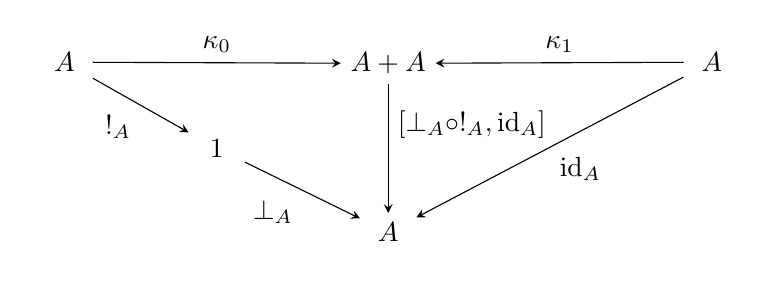
\begin{tikzpicture}
\matrix (m) [matrix of math nodes,row sep=1.7em,column sep=3.5em,minimum width=2em]
  {
     A & {} & A + A & {} & A \\
     {} & 1 \\
     {} & {} & A \\
  };
  \path[-stealth]
    (m-1-1) edge node [below left] {$!_A$} (m-2-2)
            edge node [above] {$\kappa_0$} (m-1-3)
    (m-1-3) edge node [above right] {$[\bot_A \circ !_A,\text{id}_A]$} (m-3-3)
    (m-1-5) edge node [above] {$\kappa_1$} (m-1-3)
            edge node [below right] {$\text{id}_A$} (m-3-3)
    (m-2-2) edge node [below left] {$\bot_A$} (m-3-3)
    ;
\end{tikzpicture}
\end{center}
The diagram commutes, and together with $\kappa_0 = \kappa_1$ we get $\bot_A
\circ !_A = \text{id}_A$. Furthermore, because $1$ is terminal, we have $!_A
\circ \bot_A = \text{id}_1$. We conclude that $A \cong 1$ for every $A$.
\end{proof}

\begin{proof}
(Proposition \ref{propCCCNoFixpointCoproducts}) In a CCC with binary coproducts,
$1+1$ exists. Apply \ref{propCCCWith11IsTrivial}.
\end{proof}

The singleton set $\set{\bot}$ is not initial in Cppo, because morphisms don't
preserve all cppo structure. Continuous functions must preserve lubs, but are
allowed to map $\bot$ to elements other that $\bot$. Otherwise the fixpoint
theorem would hold trivially, not giving rise to fixpoint semantics of recursive
equations.

Propositions \ref{propCCCNoFixpointInitialObject} and
\ref{propCCCNoFixpointCoproducts} are due to Huwig \cite{Huwig1990}, and
demonstrate that if we want to use Cppo, or in fact any CCC with fixpoints,  as
model for programming languages, we won't get interpretations for sum types that
correspond to categorical coproducts. Nevertheless, we have similar
constructions that serve our purpose.

The disjoint union of cppos fails to have a bottom element, thus it is not a
cppo. There are two common ways to remedy this situation. We can either use a
construction that artificially adds a new bottom element below the disjoint
union, or one that identifies all bottom elements. This is standard practice in
domain theory, see for example \cite{Gunter1992}. The former is called
\emph{separated sum}, the latter \emph{coalesced sum}.  Figure
\ref{figSeparatedAndCoalescedSum} sketches both these constructions of two given
cppos.

\begin{figure}[ht]
\begin{center}

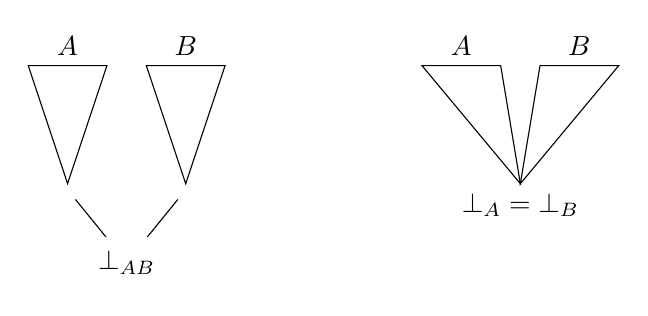
\begin{tikzpicture}[scale=1]
\draw (0,0) -- (0.5,0) node [above] {$A$} -- (1,0) -- (0.5,-1.5) -- cycle;
\begin{scope}[xshift=1.5cm]
\draw (0,0) -- (0.5,0) node [above] {$B$} -- (1,0) -- (0.5,-1.5) -- cycle;
\end{scope}
\draw[shape=rectangle] (0.6,-1.7) -- (1.25,-2.5)
  node [fill=white,inner sep=5pt] {$\bot_{AB}$} -- (1.9,-1.7)
;

\begin{scope}[xshift=5cm]
\draw (0,0) -- (0.5,0) node [above] {$A$} -- (1,0) -- (1.25,-1.5) -- cycle;
\begin{scope}[xshift=1.5cm]
\draw (0,0) -- (0.5,0) node [above] {$B$} -- (1,0) -- (-0.25,-1.5)
  node [below] {$\bot_A = \bot_B$}
  -- cycle;
\end{scope}
\end{scope}

\end{tikzpicture}

\end{center}
\caption{Separated and coalesced sum of two cppos.} \label{figSeparatedAndCoalescedSum}
\end{figure}

\begin{definition} \label{defCoalescedSum}
For objects $A$, $B$ in Cppo, define the \emph{coalesced sum} $A \oplus B$ as
the disjoint union $A \dot\cup B$ where we identify the bottom elements.
\end{definition}

\begin{definition} \label{defSeparatedSum}
For objects $A$, $B$ in Cppo, define the \emph{separated sum} $A + B$ as $A
\dot\cup B \cup \bot_{AB}$ where $\bot_{AB} \not\in A \dot\cup B$ and $\bot_{AB}
\below \bot_A$ and $\bot_{AB} \below \bot_B$.
\end{definition}

Both constructions yield cppos and their inclusions are continuous.  Both
constructions are useful for programming language semantics, as seen in section
\ref{secAlgebraicDataTypeSemantics}.  We concentrate on the separated sum for
now, because it will be important for us later on.

As seen in \ref{propCCCNoFixpointCoproducts}, the separated sum cannot be a
categorical coproduct. Consider the usual coproduct diagram in Cppo in
figure \ref{figCoproductDiagram}. For arrows $f$ and $g$,
there might be different functions $A+B \arr D$ making the diagram commute:
$\bot_{AB}$ is not in the image of the inclusions, so a function $A+B \arr D$
may map $\bot_{AB}$ to any element in $D$.  The strict function $[f\!,g]$
defined as
\begin{equation*}
[f\!,g] = x \mapsto \left\{
  \begin{array}{lcl}
   \bot   & \text{if} & x = \bot \\
   f(x')  & \text{if} & x = \kappa_0(x') \\
   g(x')  & \text{if} & x = \kappa_1(x')
  \end{array}
\right.
\end{equation*}
does make the diagram commute, and it is canonical in the sense that it
works for all $A$, $B$ and $D$.

\begin{figure}[ht]
\begin{center}
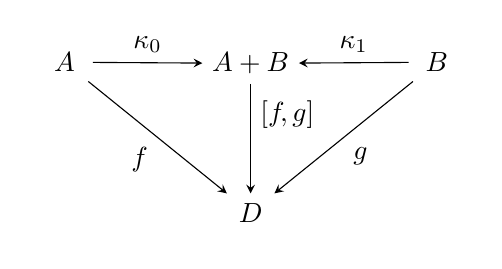
\begin{tikzpicture}[scale=1.2]
\matrix (m) [matrix of math nodes,row sep=4em,column sep=4em,minimum width=2em]
  {
     A & A + B & B \\
     {} & D & {} \\
  };
  \path[-stealth]
    (m-1-1) edge node [below left] {$f$} (m-2-2)
            edge node [above] {$\kappa_0$} (m-1-2)
    (m-1-2) edge node [above right] {$[f\!,g]$} (m-2-2)
    (m-1-3) edge node [above] {$\kappa_1$} (m-1-2)
            edge node [below right] {$g$} (m-2-2)
    ;
\end{tikzpicture}
\end{center}
\caption{The usual coproduct diagram} \label{figCoproductDiagram}
\end{figure}

While the separated sum is not a categorical coproduct, it is still a
useful construction and we can work with it as long as we keep in mind that
$[f\!,g]$ doesn't have the universal mapping property. In particular, Cppo is
closed under the separated sum construction. In fact, it is a functor.


\begin{definition}
A \emph{bifunctor} is a functor with two arguments. Formally, $F : \bbC \times \bbD \arr
\bbE$ is a bifunctor iff it is functorial in $\bbC$ and $\bbD$ separately, that
is for all fixed $C \in \bbC$ and $D \in \bbD$, both $F_C(D) = F(C \times D) : \bbD
\arr \bbE$ and $F_D(C) = F(C \times D) : \bbC \arr \bbE$ must be functors.
Furthermore, for arrows $f : C \arr C'$ in $\bbC$ and $g : D \arr D'$ in $\bbD$,
we must have the diagram commute
\begin{center}
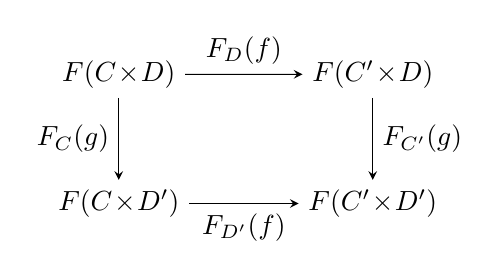
\begin{tikzpicture}
\matrix (m) [matrix of math nodes
            ,row sep=3em
            ,column sep=4em
            ,minimum width=2em]
  {
     F(C \product D) & F(C' \product D) \\
     F(C \product D') & F(C' \product D') \\
  };
  \path[-stealth]
    (m-1-1) edge node [left] {$F_C(g)$} (m-2-1)
    (m-1-1) edge node [above] {$F_D(f)$} (m-1-2)
    (m-2-1) edge node [below] {$F_{D'}(f)$} (m-2-2)
    (m-1-2) edge node [right] {$F_{C'}(g)$} (m-2-2)
    ;
\end{tikzpicture}
\end{center}
where
\begin{IEEEeqnarray*}{rCl}
F_D(f : C \arr C') & = & F(f \times 1_D) : F(C \times D) \arr F(C' \times D) \\
F_C(g : D \arr D') & = & F(1_C \times g) : F(C \times D) \arr F(C \times D')
\end{IEEEeqnarray*}
\end{definition}

\begin{proposition}

The separated sum construction is a bifunctor $+ : \Cppo \times
\Cppo \arr \Cppo$. That is for fixed $D$, the
object mapping $L_D : A \mapsto A + D$ extends to a functor: $f \mapsto
[\kappa_0 \circ f, \kappa_1 \circ \text{id}_D]$.  Symmetrically
for $R_D : A \mapsto D + A$, and we have for all $f
: A \arr A'$ and $g : B \arr B'$ the following diagram commutes.
\begin{center}
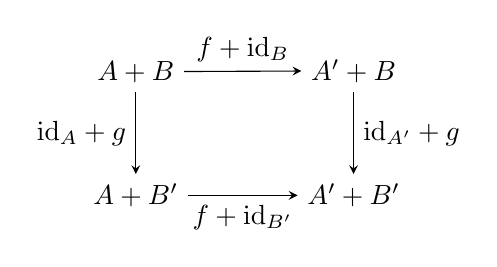
\begin{tikzpicture}
\matrix (m) [matrix of math nodes
            ,row sep=3em
            ,column sep=4em
            ,minimum width=2em]
  {
     A + B & A' + B \\
     A + B' & A' + B' \\
  };
  \path[-stealth]
    (m-1-1) edge node [above] {$f + \text{id}_B$} (m-1-2)
    (m-1-1) edge node [left] {$\text{id}_A + g$} (m-2-1)
    (m-2-1) edge node [below] {$f + \text{id}_{B'}$} (m-2-2)
    (m-1-2) edge node [right] {$\text{id}_{A'} + g$} (m-2-2)
    ;
\end{tikzpicture}
\end{center}

\end{proposition}

This sets up the stage for our following considerations.



\section{Fixpoint Semantics for Recursive Functions}
\label{secFixpointSemantics}

Using the constructions seen so far, we can show that certain recursive
functions are well-defined. This is the central idea of Scott's fixpoint
semantics for recursive programs, but it can also be employed for mathematical
purposes that don't concern programming.

First, we look at the factorial function, as it is a simple example that nicely
demonstrates the technique at work.

\begin{lemma} \label{lemPartialFunctionSpaceCppo}

Let $A, B$ be sets. The set of partial functions from $A$ to $B$, denoted
$[A \pfun B]$, is a cppo.

\end{lemma}

\begin{proof}

Let $f, g : A \pfun B$. Define $f \below g$ iff $f \subseteq g$, where we
consider $f$ and $g$ as their underlying graphs.

The totally undefined function $\emptyset = \bot$ is an element of $[A \pfun B]$
and satisfies $\bot \below g$ for all $g$.

If $F$ is a chain of functions, consider $\bigcup F$, the union of the graphs of
all functions in $F$. We have: if $f \in F$ then $f \subseteq \bigcup F$, so $f
\below \bigcup F$.  In other words $\bigcup F$ is an upper bound of $F$.

Furthermore if $g$ is an upper bound of $F$ then $\forall f \in F \ldotp f
\below g$, so $\bigcup F \below g$. In other words $\bigcup F$ is the lub of $F$
and it is justified to write $\lub F$.
\end{proof}


The definition of $f \below g$ is equivalent to the following formula, which is
less easy to read, but lends itself better to proofs.
\begin{equation*}
\forall a \in A \ldotp f(a)\isdefined \implies g(a)\isdefined\
\wedge\ f(a) = g(a)
\end{equation*}
Where $f(a)\isdefined$ is to be read as ``$f$ is defined at $a$''.

The following two lemmas are always useful for proving continuity.

\begin{lemma} \label{lemMonotoneAlwaysBelowLub}
Let $A, B$ be cpos, $f : A \arr B$ be a monotone function, and $C \subseteq A$
be a chain in A. Then $\lub f(C) \below f(\lub C)$.
\end{lemma}

\begin{proof}
We have:
\begin{IEEEeqnarray*}{rCl+x*}
           && \forall a \in C \ldotp a \below \lub C \\
 & \implies & \forall a \in C \ldotp f(a) \below f(\lub C) \\
 & \implies & f(\lub C) \text{ is an upper bound of } f(C) \\
 & \implies & \lub f(C) \below f(\lub C) & \qedhere
\end{IEEEeqnarray*}
\end{proof}


\begin{lemma} \label{lemMonotoneIsContinuousFinite}
Let $A, B$ be cpos, $f : A \arr B$ be a monotone function, and $C \subseteq A$
be a finite chain in $A$. Then $f(\lub C) = \lub f(C)$.
\end{lemma}

\begin{proof}
We have $\lub C \in C$, because $C$ is finite. Therefore $f(\lub C) \in f(C)$,
and thus $f(\lub C) \below \lub f(C)$. Lemma \ref{lemMonotoneAlwaysBelowLub}
gives the converse direction.
\end{proof}




\begin{proposition} \label{propFactorialExists}

There exists a function $f : \bbN \arr \bbN$ such that
\begin{IEEEeqnarray}{rCl}
f(0) & = & 1 \label{eqnFactorial1} \\
f(n) & = & n \cdot f(n - 1) \quad\text{if}\ \ n > 0 \label{eqnFactorial2}
\end{IEEEeqnarray}

\end{proposition}

Proposition \ref{propFactorialExists} can be rephrased in different ways: the
recursive definition of the factorial function is not vacuous; it is not a
circular definition; it does not lead to infinite regress.

\begin{proof}
From \ref{lemPartialFunctionSpaceCppo} we know that $[\bbN \pfun
\bbN]$ is a cppo. Consider the function

\begin{equation*}
\varphi(g) = n \mapsto \left\{
  \begin{array}{lcl}
   1          & \text{if} & n = 0 \\
   n \cdot g(n-1) & \text{if} & n > 0
  \end{array}
\right.
\end{equation*}

$\varphi$ is not defined recursively, so it certainly is a function $[\bbN
\pfun \bbN] \arr [\bbN \pfun \bbN]$. If we can show that
$\varphi$ is continuous, then it is an arrow in Cppo, so by theorem
\ref{thmFixpoint} it has a fixpoint $f$ such that
\begin{IEEEeqnarray}{rCl}
f = \varphi(f) \label{eqnFactorialFixpoint}
\end{IEEEeqnarray}

Using equation (\ref{eqnFactorialFixpoint}) we proceed to show that the required
equations (\ref{eqnFactorial1}) and (\ref{eqnFactorial2}) hold:
\begin{IEEEeqnarray*}{rCl}
f(0) & = & \varphi(f)(0) = 1 \\
f(n) & = & \varphi(f)(n) = n \cdot f(n - 1) \quad\text{if}\ \ n > 0
\end{IEEEeqnarray*}

We still need to show that $\varphi$ is continuous. For that matter, first
observe that $\varphi$ is monotone: assume $f \below g$. To prove: $\varphi(f)
\below \varphi(g)$, i.e.
\begin{equation*}
\forall n \in \bbN \ldotp \varphi(f)(n)\isdefined \implies
\varphi(g)(n)\isdefined\ \wedge\ \varphi(f)(n) = \varphi(g)(n)
\end{equation*}
Let $n \in \bbN$.  Assume that
$\varphi(f)(n)\isdefined$.

If $n = 0$ then $\varphi(f)(n) = 1 = \varphi(g)(n)$.

If $n > 0$ then $\varphi(f)(n) = n \cdot
f(n - 1)$. As $\varphi(f)(n)\isdefined$, we must have
$f(n-1)\isdefined$, which by assumption implies $g(n-1)\isdefined \wedge\
f(n-1) = g(n-1)$, and thus $n \cdot f(n-1) = n \cdot g(n-1) = \varphi(g)(n)$.

In both cases, $\varphi(g)(n)\isdefined \wedge\ \varphi(f)(n) = \varphi(g)(n)$,
so $\varphi(f) \below \varphi(g)$, which proves that $\varphi$ is monotone.

It remains to show that $\varphi$ preserves lubs. Let $C$ be a chain in
$[\bbN \pfun \bbN]$. Then, because $\varphi$ is monotone,
$\varphi(C)$ is a chain as well, and both have lubs $\lub C$, $\lub \varphi(C)$.
To prove: $\varphi(\lub C) = \lub \varphi(C)$. It suffices to show inequality
$\below$ in both directions.

$\lub \varphi(C) \below \varphi(\lub C)$: By lemma
\ref{lemMonotoneAlwaysBelowLub}.

$\varphi(\lub C) \below \lub \varphi(C)$: For this direction, we have to delve
into $\varphi$. It suffices to show
\begin{equation*}
  \forall n \in \bbN \ldotp \varphi(\lub C)(n)\isdefined \implies
  (\lub \varphi(C))(n)\isdefined\ \wedge\ \varphi(\lub C)(n) = (\lub
  \varphi(C))(n)
\end{equation*}
Let $n \in \bbN$. Assume $\varphi(\lub C)(n)\isdefined$.

If $n = 0$ then $\varphi(\lub C)(0) = 1$, and we have $\forall f \in C
\ldotp \varphi(f)(0) = 1$, so $(\lub \varphi(C))(0)~= 1$.

If $n > 0$ then $\varphi(\lub C)(n) = n \cdot (\lub C)(n - 1)$, and thus from
$\varphi(\lub C)(n)\isdefined$ we get $(\lub C)(n - 1)\isdefined$. But then
there must be a $g$ in $C$ such that $g(n-1)\isdefined$ and $g(n-1) = (\lub C)(n
- 1)$. But then $n \cdot g(n-1)\isdefined$, therefore $\varphi(g)(n)\isdefined$,
which implies $(\lub \varphi(C))(n)\isdefined$ and we have:
\begin{IEEEeqnarray*}{c+x*}
(\lub \varphi(C))(n) = \varphi(g)(n) = n \cdot g(n-1) = n \cdot (\lub C)(n-1)
 = \varphi(\lub C)(n) & \qedhere
\end{IEEEeqnarray*}
\end{proof}


The strategy just employed is prototypical for proving the existence of a
recursively defined function $f$. First, find a non-recursive higher-order
function corresponding to $f$ in spirit of our $\varphi$. Then prove $\varphi$
to be continuous and show that its fixpoint fulfills the desired definition.


\chapter{Algebraic Data Types}

\section{Syntax and Semantics of Algebraic Data Types}
\label{secAlgebraicDataTypeSemantics}

In this section, we motivate our interest in certain polynomial functors.

Algebraic data types (\emph{ADT}s) allow the programmer to add new base types
besides the built-in ones to a programming language. Conceptually, ADTs are sums
of products, where the factors are either constant or recursive.  Empty products
are allowed, but sums usually need to have at least one term.

Consider for example the ADT modeling lists of integers in Haskell:

\begin{verbatim}
data IntList = Nil | Cons Int IntList
\end{verbatim}

The datatype IntList is a sum of two terms. The term Nil is the empty product
while the term Cons has one constant and one recursive factor.

Denotational semantics of programming languages depend on the reduction
strategy. More precisely, if we have an operational and a denotational semantics we would like
them to commute as in diagram \ref{figOperateDenoteSemantics}, where $P$ are
programs and $D$ is our semantic domain. We want diverging programs to denote $\bot$.

\begin{figure}[ht]
\begin{center}
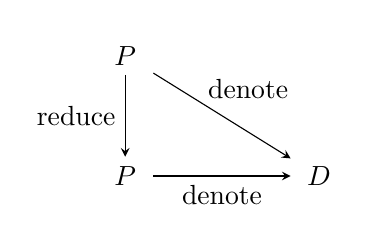
\begin{tikzpicture}
\matrix (m) [matrix of math nodes,row sep=3em,column sep=5em,minimum width=2em]
  {
     P \\
     P & D \\
  };
  \path[-stealth]
    (m-1-1) edge node [left] {reduce} (m-2-1)
    (m-1-1) edge node [above right = 1mm and -3mm] {denote} (m-2-2)
    (m-2-1.east|-m-2-2) edge node [below] {denote} (m-2-2);
\end{tikzpicture}
\end{center}
\caption{Operational and denotational semantics.}
\label{figOperateDenoteSemantics}
\end{figure}

Consider for example the program $\lambda x . 1$. When using a call-by-name evaluation
strategy we want it to denote the constant function $x \mapsto 1$. Under
call-by-value
evaluation however we would like it to denote the following function.
\begin{equation*}
x \mapsto \left\{
  \begin{array}{lcl}
   1     & \text{if} & x \neq \bot \\
   \bot  & \text{if} & x = \bot
  \end{array}
\right.
\end{equation*}
Otherwise diagram \ref{figOperateDenoteSemantics} would not commute
for the program $(\lambda x . 1)\Omega$ where $\Omega$ is some diverging
term, whose denotation is $\bot$. In general, for call-by-value evaluation
strategies we want abstractions to denote strict continuous functions, while for
call-by-name we only require continuity.

The same holds for sum and product types, and therefore for ADTs. The program
$\text{fst}\langle M,N\rangle$ for example always reduces to $M$ under a
call-by-name evaluation strategy. Call-by-value reduction however diverges if $N$ is
$\Omega$, and our denotational semantics should capture this. Technically this
means for strict evaluation we would like all pairs where at least one of the
components is $\bot$ to be identified with $\bot$. This construction is often
called the \emph{smash product}.

Similarly, the following program, which uses pseudo-code pattern matching,
diverges under call-by-value reduction, while it yields the number 1 under
call-by-name reduction.
\begin{IEEEeqnarray*}{l}
(\lambda x . \text{case}\ x\ \text{of}\\
\quad \kappa_0(-) \arr 1\\
\quad \kappa_1(-) \arr 2)\ (\kappa_0(\Omega))
\end{IEEEeqnarray*}
For denotational semantics we can use coalesced and separated sums to capture
this. In a coalesced sum of two cppos $A$ and $B$ we have $\kappa_0(\bot_A) =
\kappa_1(\bot_B) = \bot_{A \oplus B}$, while in a separated sum these are distinct
elements, which allows us to give denotations to the above program which
capture the respective termination behavior. See chapter 6 in \cite{Gunter1992}
for a more thorough treatment of sums and products under different evaluation
strategies.

The separated sum construction is not associative, that is in general we don't
have for domains $A$, $B$ and $C$ that $(A + B) + C \cong A + (B + C)$. This is
inconvenient if we want ADTs to denote sums with multiple terms. To work around
this, we use a sum construction which sums all terms simultaneously and then
adds one new bottom element, as in \cite{Manes1986}.

The empty product type arises from ADT constructors without arguments, such as
Nil in the example above. As its denotation, choosing the one-element domain for
call-by-name and the two-element domain for call-by-value
works nicely with their respective sum constructions.

The cartesian product in $\Cppo$ is a categorical product. Likewise, the
coalesced sum is a categorical coproduct in $\Cppo_\bot$. The separated sum
however is not a coproduct in $\Cppo$, and the smash product not a product in
$\Cppo_\bot$. This result, that call-by-value doesn't have products and
call-by-name doesn't have coproducts, is discussed in \cite{Filinski1989}.

We summarize above considerations in table \ref{figTableDenSem}.

\begin{figure}[ht]
\begin{center}
\begin{tabular}{c|c|c}
 & call-by-value & call-by-name \\
\hline
category & $\Cppo_{\bot}$ & $\Cppo$ \\
abstraction & strict continuous function & continuous function \\
sum type & coalesced sum & separated sum \\
product type & smash product & cartesian product \\
empty product type & 2 & 1
\end{tabular}
\end{center}
\caption{Denotational semantics for algebraic data types}
\label{figTableDenSem}
\end{figure}

\section{Naturals With And Without Computation Steps}

Section \ref{secAlgebraicDataTypeSemantics} gave the motivation for lazy
polynomial functors. In this section we look at the relationship between the
concrete functors
\begin{IEEEeqnarray*}{rCl}
FX & = & 1 + X \\
GX & = & 1 + X + X
\end{IEEEeqnarray*}
and their respective final coalgebras:
\begin{IEEEeqnarray*}{c}
\alpha : A \arr FA \\
\beta : B \arr GB
\end{IEEEeqnarray*}

The following is a well-known fact in the field of algebras and coalgebras.

\begin{lemma} \label{lemLambek}
(Lambek op) Final coalgebras are isomorphisms.
\end{lemma}

\begin{proof}
Let $F$ be a functor and $\alpha : A \arr FA$ its final coalgebra. Then $F\alpha
: FA \arr FFA$ is an $F$-coalgebra, so the coalgebra map $f : FA \arr A$ exists
such that diagram $II$ in figure \ref{figLambeksLemmaOp} commutes.

\begin{figure}[ht]
\begin{center}
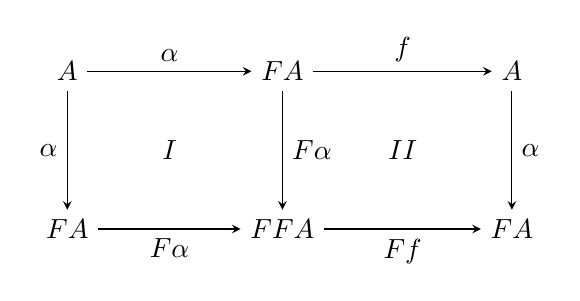
\begin{tikzpicture}
\matrix (m) [matrix of math nodes
            ,row sep=1.5em
            ,column sep=2em
            ,minimum width=1em]
  {
     A & & FA & & A \\
     & I & & II & \\
     FA & & FFA & & FA \\
  };
  \path[-stealth]
    (m-1-1) edge node [left] {$\alpha$} (m-3-1)
    (m-1-1) edge node [above] {$\alpha$} (m-1-3)
    (m-3-1) edge node [below] {$F\alpha$} (m-3-3)
    (m-1-3) edge node [right] {$F\alpha$} (m-3-3)
    (m-1-3) edge node [above] {$f$} (m-1-5)
    (m-3-3) edge node [below] {$Ff$} (m-3-5)
    (m-1-5) edge node [right] {$\alpha$} (m-3-5)
    ;
\end{tikzpicture}
\end{center}
\caption{Lambek's lemma op}
\label{figLambeksLemmaOp}
\end{figure}

Diagram $I$ commutes as well, so by finality of $\alpha$ we have $f \circ
\alpha = \text{id}_A$. Furthermore $\alpha \circ f = Ff \circ F\alpha = F(f
\circ \alpha) = F(\text{id}_A) = \text{id}_{FA}$.
\end{proof}


\begin{proposition} \label{propEpsilonPiExist}
There exists a continuous embedding-projection pair
\begin{IEEEeqnarray*}{RCCl}
\varepsilon : & A & \arr & B \\
\pi         : & B & \arr & A
\end{IEEEeqnarray*}
such that $\pi \circ \varepsilon = \text{id}_A$.
\end{proposition}


Greatest fixpoints of functors arise as limits of left chains. See theorem
11.3.14 in \cite{Manes1986}.  \begin{IEEEeqnarray*}{c}
\cdots\ \arr\ F^3(1)\ \arr\ F^2(1)\ \arr\ F(1)\ \arr\ 1
\end{IEEEeqnarray*}
Intuitively, the cppos we use for data structure semantics arise by
$\omega$-fold iteration of the base functor on the terminal object $1$. The
first few iterations for the functor $FX = 1 + X$, together with the partial
order induced by the separated sum, are illustrated in figure
\ref{figFirstIterationsOfF}. In each iteration, the cppo of the previous step is
lifted through $\kappa_1$ to the upper right, and fresh $\kappa_0(\bot)$ and
$\bot$ are introduced.


\begin{figure}
\begin{center}
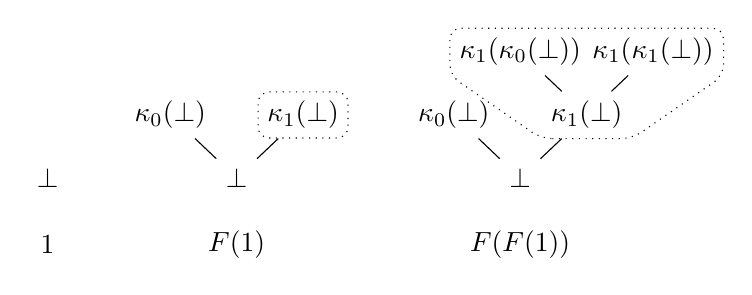
\begin{tikzpicture}[scale=1.2]
  \node {$\bot$} [grow'=up, sibling distance=4.0em, level distance=1.9em]
  ;

  \node at (0,-0.7) {$1$};

  \node at (2,0) {$\bot$} [grow'=up, sibling distance=4.0em, level distance=1.9em]
    child { node {$\kappa_0(\bot)$} }
    child { node [draw,dotted,rounded corners] {$\kappa_1(\bot)$} }
  ;

  \node at (2,-0.7) {$F(1)$};

  \node at (5,0) {$\bot$} [grow'=up, sibling distance=4.0em, level distance=1.9em]
    child { node {$\kappa_0(\bot)$} }
    child {
      node [name=foo] { $\kappa_1(\bot)$ }
      child { node [name=bar] { $\kappa_1(\kappa_0(\bot))$ } }
      child { node [name=baz] { $\kappa_1(\kappa_1(\bot))$ } }
    }
  ;

  \node at (5,-0.7) {$F(F(1))$};

  \path [draw,dotted,rounded corners] (foo.south west) -- (foo.south east)
    -- (baz.south east)
    -- (baz.north east)
    -- (bar.north west)
    -- (bar.south west)
    -- cycle
  ;

\end{tikzpicture}
\end{center}
\caption{The first iterations of $1+X$ on $1$. Marked parts indicate the
inclusion of the previous iteration.}
\label{figFirstIterationsOfF}
\end{figure}

The final coalgebras $A$ and $B$, together with their ordering are depicted in
the Hasse diagrams of figures \ref{figDomainOfLazyNaturals} and
\ref{figDomainOfNuF}. These figures employ some notational simplification.

\begin{figure}[th]
\begin{center}
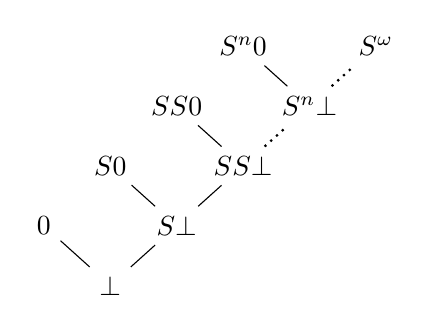
\begin{tikzpicture}[scale=1.2]
  \node {$\bot$} [grow'=up, sibling distance=4.0em, level distance=1.8em]
    child { node {$0$} }
    child
    {
      node {$S\bot$}
      child { node {$S0$} }
      child
      {
        node {$SS\bot$}
        child { node {$SS0$} }
        child [thick, dotted]
        {
          node {$S^n\bot$}
          child [thin, solid] { node {$S^n0$} }
          child { node {$S^\omega$} }
        }
      }
    }
  ;
\end{tikzpicture}
\end{center}
\caption{The cppo $(A, \below)$.}
\label{figDomainOfLazyNaturals}
\end{figure}

\begin{figure}[th]
\begin{center}
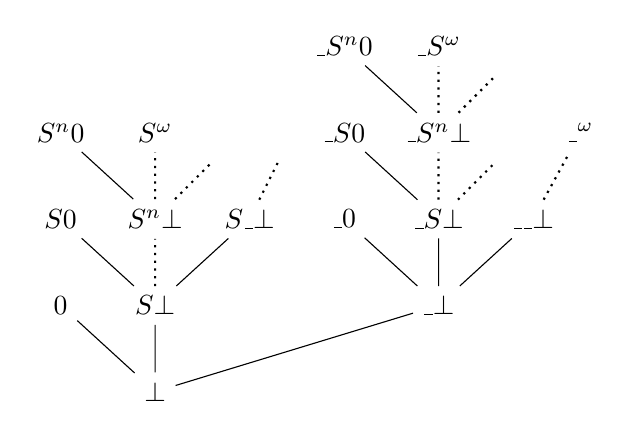
\begin{tikzpicture}
 [ grow'=up
 , scale=1.2
 , level distance=2.6em
 , level 1/.style={sibling distance=3cm}
 , level 2/.style={sibling distance=1cm}
 , normal/.style={thin, solid}
 , skipping/.style={thick, dotted}
 , and so on/.style={thick, dotted, sibling distance=0.6cm, level distance=0.6cm}
 ]
  \node {$\bot$}
    child [sibling distance=1cm] { node {$0$} }
    child
    {
      node {$S\bot$}
      child { node {$S0$} }
      child [skipping]
      {
        %node {$SS\bot$}
        %child { node {$SS0$} }
        %child [skipping]
        %{
          node {$S^n\bot$}
          child [normal] { node {$S^n0$} }
          child [skipping] { node {$S^\omega$} }
          child [and so on] {}
        %}
        %child [and so on] {}
      }
      child
      {
        node {$S\_\bot$}
        child [missing] {}
        child [and so on] {}
      }
    }
    child
    {
      node {$\_ \bot$}
      child { node {$\_0$} }
      child
      {
        node {$\_S\bot$}
        child { node {$\_S0$} }
        child [skipping]
        {
          node {$\_S^n\bot$}
          child [normal] { node {$\_S^n0$} }
          child { node {$\_S^\omega$} }
          child [and so on] {}
        }
        child [and so on] {}
      }
      child
      {
        node {$\_\_\bot$}
        child [missing] {}
        %child [missing] {}
        child [skipping] { node {$\_^\omega$} }
      }
    }
  ;
\end{tikzpicture}
\end{center}
\caption{The cppo $(B, \below)$.}
\label{figDomainOfNuF}
\end{figure}


\begin{lemma} \label{lemEpsilonExists}
There is a continuous function $\varepsilon : A \arr B$ such that

\begin{equation*}
\varepsilon(a) = \left\{
  \begin{array}{rcl}
   \bot_B & \text{if} & a = \bot_A \\
   \beta^{-1}(\kappa_0(a')) & \text{if} & \beta(a) = \kappa_0(a') \\
   \beta^{-1}(\kappa_1(\varepsilon(a'))) & \text{if} & \beta(a) = \kappa_1(a')
  \end{array}
\right.
\end{equation*}

\end{lemma}

This specification is highly technical, and it's hard to see that there really
is not much going on.  From now on we employ some notational simplifications to
make matters more clear.

First, lemma \ref{lemLambek} allows us to be liberal with $\alpha$ and $\beta$,
so we leave them out and view an element of $A$ as also being of $1 + A$ and
vice versa. Same for $B$ and $1+B+B$. When appropriate, we write ``$x$ is of the
form $S(-)$'' instead of $\exists x' \ldotp \alpha(x) = S(x')$ .

Second, $1$ as the terminal object in Cppo is a one-element set, so
$\kappa_0(a')$ can only be of the form $\kappa_0(\bot)$ for which we write
$0$.

Third, we write $S$ for $\kappa_1$ and $\_$ for $\kappa_2$.

The equation of \ref{lemEpsilonExists} then becomes:

\begin{equation*}
\varepsilon(a) = \left\{
  \begin{array}{rcl}
   \bot & \text{if} & a = \bot \\
   0 & \text{if} & a = 0 \\
   S(\varepsilon(a')) & \text{if} & a = S(a')
  \end{array}
\right.
\end{equation*}

From this it is easier to see that $\varepsilon$ doesn't do anything except
embedding a value of $1+A$ in $1+B+B$. The proof proceeds similarly to the one
of \ref{propFactorialExists}, but now we have more work to do, as we
additionally want $\varepsilon$ to be continuous. We need the following
lemmas.


\begin{lemma} \label{lemDefinitionBelowAandB}
For $x,y \in A$, we have $x \below y$ iff
\begin{IEEEeqnarray*}{rtl}
& & x = \bot \\
& or\quad & x = y \\
& or\quad & x = S(x') \aand y = S(y') \aand x' \below y'
\end{IEEEeqnarray*}

For $x,y \in B$, we have $x \below y$ iff
\begin{IEEEeqnarray*}{tlClClCl+x*}
& x = \bot \\
or\quad & x = y \\
or\quad & x = S(x') & \aand & y & = & S(y') & \aand & x' \below y' \\
or\quad & x = \_(x') & \aand & y & = & \_(y') & \aand & x' \below y' & \qed
\end{IEEEeqnarray*}
\end{lemma}


\begin{lemma} \label{lemCoFiniteSubsetLub}

If $C$ is an infinite chain and $C' \subseteq C$ a co-finite subset, then $\lub
C = \lub C'$. \qed

\end{lemma}


\begin{lemma} \label{lemChainInversion}

If $C$ is an infinite chain in $A$ such that $\lub C = S(a)$ for some $a \in A$,
then
\begin{enumerate}

  \item \label{lemChainInversion1} All but finitely many $x \in C$ are of the
  form $S(-)$.  In other words, there is a co-finite subset $C'$ of $C$ having
  the same lub, where all elements of $C'$ are of the form $S(-)$.

  \item \label{lemChainInversion2} The set $C'' = \set{x' \mid S(x') \in C'}$ is
  a chain, and $\lub C = S(\lub C'')$.
\end{enumerate}

\end{lemma}

Intuitively, this lemma states that if a chain eventually rises into $S$:
\begin{IEEEeqnarray*}{c}
\bot \below \ldots \below \bot \below S(x_0) \below S(x_1) \below S(x_2) \below \ldots
\end{IEEEeqnarray*}
then the sequence
\begin{IEEEeqnarray*}{c}
x_0 \below x_1 \below x_2 \below \ldots
\end{IEEEeqnarray*}
is a chain and the lub of the first is the same as the successor of the lub of
the second. The set $C'$ is the chain with all leading non-$S$ elements removed, and $C''$ is $\set{x_0, x_1, x_2, \ldots}$.

This lemma is similar to lemma \ref{lemMonotoneAlwaysBelowLub}, which
intuitively states that arbitrary monotone functions factor into chains, while
here $S$ factors out of chains.


\begin{proof}

(Lemma \ref{lemChainInversion}) \ref{lemChainInversion1}. Let $C$ be an infinite
chain such that $\lub C = S(a)$, and assume towards a contradiction that
infinitely many elements are not of the form $S(-)$. Then, for each $x \in C$,
there is a $y \in C$ such that $x \below y \below S(a)$ and $y$ is not of
the form $S(-)$. Then, by definition of $\below$, $y$ must be $\bot$. But
then $\bot$ is an upper bound of $C$, which contradicts the assumption that
$S(a)$ is the least upper bound of $C$.

\ref{lemChainInversion2}. We show that the order on $C''$ is total. Let $x', y'
\in C''$. Then by definition of $C''$, there are $x, y \in C'$ such that $x
\below y \aand x = S(x') \aand y = S(y')$. By lemma
\ref{lemDefinitionBelowAandB} this gives $x' \below y'$.

It remains to show that $\lub C = S(\lub C'')$. It suffices to show that $a =
\lub C''$, because then $\lub C = S(a) = S(\lub C'')$. We calculate:
\begin{IEEEeqnarray*}{rCls}
&& \forall x' \in C'' \ldotp S(x') \below S(a) & ($S(a)$ upper bound of $C'$) \\
& \implies & \forall x' \in C'' \ldotp x' \below a & (lemma \ref{lemDefinitionBelowAandB})\\
& \implies & a \text{ is an upper bound of } C''.
\end{IEEEeqnarray*}

Let $b$ be an upper bound of $C''$. Then
\begin{IEEEeqnarray*}{rClsx*}
&& \forall x' \in C'' \ldotp x' \below b \\
& \implies & \forall x' \in C'' \ldotp S(x') \below S(b) & ($S$ monotone)\\
& \implies & S(b) \text{ is an upper bound of } C' & (definition $C''$) \\
& \implies & \lub C' = S(a) \below S(b) & (S(a) least upper bound) \\
& \implies & a \below b & (lemma \ref{lemDefinitionBelowAandB}) \\
& \implies & a \text{ is the least upper bound of } C'' & & \qedhere
\end{IEEEeqnarray*}
\end{proof}

A similar result holds for a chain in $B$ which eventually rises into $S$ or
$\_$. The proof proceeds for each constructor separately, where the respective other
constructor is not relevant, so the proof works in both cases just as in
\ref{lemChainInversion}:

\begin{lemma} \label{lemChainInversionB}
If $C$ is a chain in $B$ with $\lub C = S(b)$ for some $b \in B$, then $\lub C =
S(\lub C'')$ where $C'' = \set{x \mid S(x) \in C}$. Symmetrically for $\lub C =
\_(b)$. \qed
\end{lemma}


\begin{proof}

(Lemma \ref{lemEpsilonExists}) Define $\varphi : [A \arr B] \arr [A \arr B]$ as:

\begin{equation*}
\varphi(f) = a \mapsto \left\{
  \begin{array}{rcl}
   \bot & \text{if} & a = \bot \\
   0 & \text{if} & a = 0 \\
   S(f(a')) & \text{if} & a = S(a')
  \end{array}
\right.
\end{equation*}

As we now work in Cppo, $[A \arr B]$ denotes the set of continuous functions
from $A$ to $B$. To prove:
\begin{enumerate}[noitemsep]
\item \label{proofEpsilonExists1} $\varphi$ maps continuous functions to
continuous functions.
\item \label{proofEpsilonExists2} $\varphi$ is itself continuous.
\item \label{proofEpsilonExists3} $\varepsilon$ as the fixpoint of $\varphi$
satisfies the desired equation.
\end{enumerate}

\ref{proofEpsilonExists1}. Let $f : A \arr B$ be continuous. We have to show
that $\varphi(f)$ is monotone and preserves lubs.

Monotonicity: let $x, y \in A$ such that $x \below y$.

If $x = \bot$ then $\varphi(f)(x) = \bot \below \varphi(f)(y)$ always.

If $x = 0$ then $y = 0$ as well, so $\varphi(f)(x) = \varphi(f)(y)$.

If $x = S(x')$ then, because $x \below y$ and lemma \ref{lemDefinitionBelowAandB}, there must be a $y'$ such that $y =
S(y')$ and $x' \below y'$. But $S$ and $f$ are both monotone, so
\begin{equation*}
\varphi(f)(x) = S(f(x')) \below S(f(y')) = \varphi(f)(y).
\end{equation*}

Lub preservation: Let $C$ be a chain in $A$. To prove: $\varphi(f)(\lub C) =
\lub \varphi(f)(C)$.

If $\lub C = \bot$ then $C$ is finite, and the conclusion follows by lemma
\ref{lemMonotoneIsContinuousFinite}.

If $\lub C = 0$ then again $C$ must be finite.

If $\lub C = S(a)$ for some $a \in A$ then if $C$ is finite, we're done. Let $C$
be infinite. Using lemma \ref{lemChainInversion} and its constructions
$C'$ and $C''$, we calculate:
\begin{IEEEeqnarray*}{rCl's}
&& \varphi(f)(\lub C) \\
& = & \varphi(f)(S(a)) \\
& = & S(f(a)) & (definition $\varphi$) \\
& = & S(f(\lub C'')) & (lemma \ref{lemChainInversion}) \\
& = & \lub S(f(C'')) & ($S, f$ continuous) \\
& = & \lub \varphi(f)(S(C'')) & (definition $\varphi$) \\
& = & \lub \varphi(f)(C') & (definition $C'$) \\
& = & \lub \varphi(f)(C) & (lemma \ref{lemCoFiniteSubsetLub})
\end{IEEEeqnarray*}

\ref{proofEpsilonExists2}. Monotonicity: Let $f,g \in [A \arr B]$ such that $f
\below g$.  To prove: $\varphi(f) \below \varphi(g)$, i.e. $\forall a \in A
\ldotp \varphi(f)(a) \below \varphi(g)(a)$.  The cases $a = \bot$ and $a = 0$
are straight forward, so let $a = S(a')$. Then
\begin{IEEEeqnarray*}{c}
\varphi(f)(a) = S(f(a')) \below S(g(a')) = \varphi(g)(a).
\end{IEEEeqnarray*}

Lub preservation: Let $C = \set{f_n \mid n \in \bbN}$ be a chain
in $[A \arr B]$.  To prove: $\varphi(\lub C) = \lub \varphi(C)$. Let $a \in
A$. Because lubs of function chains are defined pointwise, it suffices to show
$\lub \varphi(C)(a) = \varphi(\lub C)(a)$.

If $a = \bot$ then $\varphi(f)(a) = \bot$ for all $f \in C$, so
\begin{IEEEeqnarray*}{c}
    \lub \varphi(C)(a)
  = \lub \set{\bot}
  = \bot
  = \varphi(\lub C)(a).
\end{IEEEeqnarray*}

If $a = 0$ then $\varphi(f)(a) = 0$ for all $f \in C$, so
\begin{IEEEeqnarray*}{c}
    \lub(\varphi(C)(a))
  = \lub \set{0}
  = 0
  = \varphi(\lub C)(0).
\end{IEEEeqnarray*}

If $a = S(a')$ then
\begin{IEEEeqnarray*}{rClu}
     && \lub(\varphi(C)(a)) \\
  & = & \lub \set{S(f_n(a')) \mid n \in \bbN} & (definition of $\varphi$) \\
  & = & S(\lub \set{f_n(a') \mid n \in \bbN}) & (S is continuous) \\
  & = & S((\lub C)(a')) & (lubs are defined pointwise) \\
  & = & \varphi(\lub C)(a) & (definition of $\varphi$)
\end{IEEEeqnarray*}

Now we know that $\varphi$ is continuous, so we use the fixpoint theorem to
conclude that $\varphi$ has a least fixpoint, call it $\varepsilon$. It remains
to show that $\varepsilon$ has the desired properties.

\ref{proofEpsilonExists3}. We have $\varepsilon = \varphi(\varepsilon)$. Let $a
\in A$.

If $a = \bot$ then $\varepsilon(a) = \varphi(\varepsilon)(a) = \bot$.

If $a = 0$ then $\varepsilon(a) = \varphi(\varepsilon)(a) = 0$.

If $a = S(a')$ then $\varepsilon(a) = \varphi(\varepsilon)(a) =
S(\varepsilon(a'))$.
\end{proof}

The proof that $\pi$ exists and has the desired properties follows the same
sche\-ma as for $\varepsilon$, except we have one more case to consider. We leave out all the
boilerplate and concentrate on the interesting cases.

\begin{lemma} \label{lemPiExists}
There is a function $\pi : B \arr A$ such that

\begin{IEEEeqnarray*}{c}
\pi(b) = \left\{
  \begin{array}{rcl}
   \bot & \text{if} & b = \bot \\
   0 & \text{if} & b = 0 \\
   S(\pi(b')) & \text{if} & b = S(b') \\
   \pi(b') & \text{if} & b = \_(b')
  \end{array}
\right.
\end{IEEEeqnarray*}

\end{lemma}

\begin{proof}
(Lemma \ref{lemPiExists}) Define $\psi : [B \arr A] \arr [B \arr A]$ as:

\begin{IEEEeqnarray*}{c}
\psi(f) = b \mapsto \left\{
  \begin{array}{rcl}
   \bot & \text{if} & b = \bot \\
   0 & \text{if} & b = 0 \\
   S(f(b')) & \text{if} & b = S(b') \\
   f(b') & \text{if} & b = \_(b')
  \end{array}
\right.
\end{IEEEeqnarray*}

To prove:
\begin{enumerate}[noitemsep]
\item \label{proofPiExists1} $\psi$ maps continuous functions to
continuous functions.
\item \label{proofPiExists2} $\psi$ is itself continuous.
\item \label{proofPiExists3} $\pi$ as the fixpoint of $\psi$
satisfies the desired equation.
\end{enumerate}

\ref{proofPiExists1}. Let $f \in [B \arr A]$. To prove: $\psi(f)$ is continuous.

Monotonicity: Let $x,y \in B$ such that $x \below y$.

If $x = S(x')$ then by lemma \ref{lemDefinitionBelowAandB} there must be a $y'$
such that $y = S(y')$ and $x' \below y'$. We have:
\begin{IEEEeqnarray*}{c}
\psi(f)(x) = S(f(x')) \below S(f(y')) = \psi(f)(y).
\end{IEEEeqnarray*}

If $x = \_(x')$ then there must be a $y'$ such that $y = \_(y')$ and $x' \below
y'$. We have:
\begin{IEEEeqnarray*}{c}
\psi(f)(x) = f(x') \below f(y') = \psi(f)(y).
\end{IEEEeqnarray*}


Lub preservation: Let $C$ be a chain in $B$. To prove: $\psi(f)(\lub
C) = \lub \psi(f)(C)$.

If $C$ is infinite and $\lub C = S(b)$ for some $b \in B$, then:
\begin{IEEEeqnarray*}{rCl's}
&&    \psi(f)(\lub C) \\
& = & \psi(f)(S(b)) \\
& = & S(f(b)) & (def. $\psi$) \\
& = & S(f(\lub C'')) & (lemma \ref{lemChainInversionB}) \\
& = & \lub S(f(C'')) & ($S$, $f$ continuous) \\
& = & \lub \psi(f)(S(C'')) & (def. $\psi$) \\
& = & \lub \psi(f)(C') & (def. $C''$) \\
& = & \lub \psi(f)(C) & (lemma \ref{lemCoFiniteSubsetLub})
\end{IEEEeqnarray*}

If $C$ is infinite and $\lub C = \_(b)$ for some $b \in B$, then:
\begin{IEEEeqnarray*}{rCl's}
&&    \psi(f)(\lub C) \\
& = & \psi(f)(\_(b)) \\
& = & f(b) \\
& = & f(\lub C'') & (lemma \ref{lemChainInversionB}) \\
& = & \lub f(C'') \\
& = & \lub \psi(f)(\_(C'')) \\
& = & \lub \psi(f)(C') \\
& = & \lub \psi(f)(C)
\end{IEEEeqnarray*}

\ref{proofPiExists2}. Monotonicity: Let $f, g \in [B \arr A]$ such that $f
\below g$. To prove: $\psi(f) \below \psi(g)$, which is equivalent to $\forall b
\in B \ldotp \psi(f)(b) \below \psi(g)(b)$. Let $b \in B$.

If $b = S(b')$ then
\begin{IEEEeqnarray*}{c}
\psi(f)(b) = S(f(b')) \below S(g(b')) = \psi(g)(b).
\end{IEEEeqnarray*}

If $b = \_(b')$ then
\begin{IEEEeqnarray*}{c}
\psi(f)(b) = f(b') \below g(b') = \psi(g)(b).
\end{IEEEeqnarray*}

Lub preservation: Let $C$ be a chain in $[B \arr A]$. To prove: $\psi(\lub C) =
\lub \psi(C)$. Lubs of function chains are defined pointwise, so it suffices to
show that $\forall b \in B \ldotp \psi(\lub C)(b) = \lub(\psi(C)(b))$. Let $b
\in B$.

If $b = S(b')$ then
\begin{IEEEeqnarray*}{rClu}
     && \lub(\psi(C)(b)) \\
  & = & \lub \set{S(f_n(b')) \mid n \in \bbN} & (definition of $\psi$) \\
  & = & S(\lub \set{f_n(b') \mid n \in \bbN}) & (S is continuous) \\
  & = & S((\lub C)(b')) & (lubs are defined pointwise) \\
  & = & \psi(\lub C)(b) & (definition of $\psi$)
\end{IEEEeqnarray*}

If $b = \_(b')$ then
\begin{IEEEeqnarray*}{rClu}
     && \lub(\psi(C)(b)) \\
  & = & \lub \set{f_n(b') \mid n \in \bbN} & (definition of $\psi$) \\
  & = & (\lub C)(b') & (lubs are defined pointwise) \\
  & = & \psi(\lub C)(b) & (definition of $\psi$)
\end{IEEEeqnarray*}

By the fixpoint theorem, $\psi$ has a least fixpoint $\pi$. We have $\pi =
\psi(\pi)$, and we still need to prove the equation of the lemma.

\ref{proofPiExists3}. Let $b \in B$.

If $b = \bot$ then $\pi(b) = \psi(\pi)(b) = \bot$.

If $b = 0$ then $\pi(b) = \psi(\pi)(b) = 0$.

If $b = S(b')$ then $\pi(b) = \psi(\pi)(b) = S(\pi(b'))$.

If $b = \_(b')$ then $\pi(b) = \psi(\pi)(b) = \pi(b')$.
\end{proof}

We are now ready to conclude the result of this section.

\begin{proof}
(Proposition \ref{propEpsilonPiExist}) The existence of $\varepsilon$ and $\pi$
was proven in lemmas \ref{lemEpsilonExists} and \ref{lemPiExists}. To show that
they form an embedding-projection-pair, i.e. $\pi \circ \varepsilon =
\text{id}_A$, let $a \in A$.

If $a = \bot$ then $\pi(\varepsilon(\bot)) = \pi(\bot) = \bot$.

If $a = 0$ then $\pi(\varepsilon(0)) = \pi(0) = 0$.

If $a = S(a')$ then $\pi(\varepsilon(S(a'))) = \pi(S(\varepsilon(a'))) =
S(\pi(\varepsilon(a')))$.

In all cases, $\alpha \circ (\pi \circ \varepsilon) = F(\pi \circ \varepsilon)
\circ \alpha$, which means that the following diagram commutes, and because
$\alpha$ is the final coalgebra for $F$ this implies $\pi \circ \varepsilon =
\text{id}_A$.
\end{proof}
\begin{figure}[h]
\begin{center}
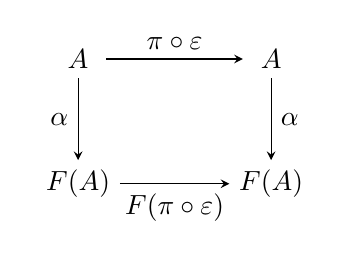
\begin{tikzpicture}
\matrix (m) [matrix of math nodes,row sep=3em,column sep=4em,minimum width=2em]
  {
     A & A \\
     F(A) & F(A) \\
  };
  \path[-stealth]
    (m-1-1) edge node [left] {$\alpha$} (m-2-1)
            edge node [above] {$\pi \circ \varepsilon$} (m-1-2)
    (m-2-1.east|-m-2-2) edge node [below] {$F(\pi \circ \varepsilon)$} (m-2-2)
    (m-1-2) edge node [right] {$\alpha$} (m-2-2);
\end{tikzpicture}
\end{center}
\end{figure}

For the other direction it would be nice to have at least $\varepsilon \circ
\pi \below \text{id}_B$, but that's not the case. To see why,
consider the counterexample
\begin{IEEEeqnarray*}{rCl}
\varepsilon(\pi(\_S0)) = \varepsilon(S0) = S0
\end{IEEEeqnarray*}
where $\_S0$ and $S0$ are not related by $\below$ in $B$.

\section{Generalization of the Construction}

\begin{lemma} \label{lemFunctionCompositionContinuous}
Function composition
\begin{IEEEeqnarray*}{c}
\circ : [A \arr B] \times [B \arr C] \arr [A \arr C]
\end{IEEEeqnarray*}
is continuous. See \cite{Gunter1992} p.123. \qed
\end{lemma}


\begin{lemma} \label{lemLubSumPointwise}
For $\set{f_i}$, $\set{g_j}$ chains of functions in $[A \arr C]$ and $[B \arr
C]$ respectively, we have:
\begin{IEEEeqnarray*}{c}
[\lub \set{f_i}, \lub \set{g_j}] = \lub \set{[f_i, g_i]} : A+B \arr C
\end{IEEEeqnarray*}
\end{lemma}

\begin{proof}
For $x \in A+B$ we have:

If $x = \bot$ then $[\lub \set{f_i}, \lub \set{g_j}](\bot) = \bot = \lub
\set{[f_i,g_i](\bot)} = \lub \set{[f_i,g_i]}(\bot)$.

If $x = \kappa_0(a)$ then:
\begin{IEEEeqnarray*}{rCl"s} %"
[\lub \set{f_i}, \lub \set{g_j}](\kappa_0(a))
  & = & (\lub \set{f_i})(a)  & (def. $[-,-])$\\
  & = & \lub \set{f_i(a)}  & (def. lubs of function chains)\\
  & = & \lub \set{[f_i, g_i](\kappa_0(a))} & (def $[-,-]$\\
  & = & \lub \set{[f_i, g_i]} (\kappa_0(a)) & (def. lubs of function chains)
\end{IEEEeqnarray*}
If $x = \kappa_1(b)$, analogous to the previous case.
\end{proof}

\begin{definition}
A functor $F : \Cppo \arr \Cppo$ is called \emph{polynomial} iff it is of one of the following forms.
\begin{itemize}[noitemsep]
\item F is a constant functor $FX = D$, $Ff = id_D$ for some $D$.
\item F is the identity functor $FX = X$, $Ff = f$.
\item F is a product $FX = GX \product HX$ where $G$, $H$ are polynomial.
\item F is a separated sum $FX = GX + HX$ where $G$, $H$ are polynomial.
\end{itemize}
\end{definition}

As discussed in section \ref{secAlgebraicDataTypeSemantics}, the separated sum
is not associative. We can work around this by allowing our separated sums to
have many terms simultaneously, that is $FX = G_0X + G_1X + \ldots + G_nX$ where
all $G_i$ are polynomial. The disjoint union is then taken of all the terms
simultaneously, and one new bottom element is introduced below the result. The
following proofs work just the same for such sums, apart from an induction on
the number of terms.

\begin{lemma} \label{lemPolynomialFunctorsContinuous}
Polynomial functors are continuous on arrows. That is, if $F : \Cppo \arr \Cppo$
is a polynomial functor and $C = \set{f_i}$ a chain in some function space $[A
\arr B]$, then $F(\lub C) = \lub FC$, where $FC = \set{Ff_i}$.
\end{lemma}

\begin{proof}
By induction on $F$. If $F$ is a constant functor $F(X) = D$, $Ff = \text{id}_D$
then
\begin{IEEEeqnarray*}{c}
\lub \set{Ff_i} = \lub \set{\text{id}_D} = \text{id}_D = F(\lub C).
\end{IEEEeqnarray*}

If $F$ is the identity functor $F(X) = X$, $Ff = f$ then
\begin{IEEEeqnarray*}{c}
\lub \set{Ff_i} = \lub \set{f_i} = F(\lub C).
\end{IEEEeqnarray*}

If $F$ is a product the form $FX = GX \product HX$ for continuous $G$ and $H$,
we have:
\begin{IEEEeqnarray*}{rCl"s} %" auto-completion fuckup: closing quote
F(\lub C) & = & G(\lub C) \product H(\lub C) \\
  & = & \langle G(\lub C) \circ \pi_1, H(\lub C) \circ \pi_2 \rangle
             & (def. $\times$) \\
  & = & \langle \lub GC \circ \pi_1, \lub HC \circ \pi_2 \rangle
             & (induction hypothesis)\\
  & = & \langle \lub \set{Gf_i} \circ \pi_1, \lub \set{Hf_j} \circ \pi_2 \rangle \\
  & = & \langle \lub \set{Gf_i \circ \pi_1}, \lub \set{Hf_j \circ \pi_2} \rangle
             & (lemma \ref{lemFunctionCompositionContinuous}) \\
  & = & \lub \set{ \langle Gf_i \circ \pi_1, Hf_i \circ \pi_2 \rangle }
             & (def. lubs in products) \\
  & = & \lub \set{ Gf_i \product Hf_i } \\
  & = & \lub \set{ Ff_i } = \lub FC
\end{IEEEeqnarray*}

If $F$ is a separated sum of the form $FX = GX + HX$ for continuous $G$ and $H$,
we have:
\begin{IEEEeqnarray*}{rCl"sx*} %"
F(\lub C) & = & G(\lub C) + H(\lub C) \\
  & = & [\kappa_0 \circ G(\lub C), \kappa_1 \circ H(\lub C)] \\
  & = & [\kappa_0 \circ \lub \set{Gf_i}, \kappa_1 \circ \lub \set{Hf_j}]
              & (induction hypothesis) \\
  & = & [\lub \set{\kappa_0 \circ Gf_i}, \lub \set{\kappa_1 \circ Hf_j}]
              & (lemma \ref{lemFunctionCompositionContinuous}) \\
  & = & \lub \set{[\kappa_0 \circ Gf_i, \kappa_1 \circ Hf_i]}
              & (lemma \ref{lemLubSumPointwise}) \\
  & = & \lub \set{Ff_i} = \lub FC && \qedhere
\end{IEEEeqnarray*}
\end{proof}

\begin{definition}
Let $F : \Cppo \arr \Cppo$ be a polynomial functor. Then $G(X) = F(X) + X$ is a
polynomial functor as well. Let $\alpha : A \arr FA$ and $\beta : B \arr GB$
be their respective final coalgebras.
\end{definition}

\begin{proposition}
There exist $\varepsilon : A \arr B$ and $\pi : B \arr A$ such that $\pi
\circ \varepsilon = \text{id}_A$
\end{proposition}

\begin{proof}

Define
\begin{IEEEeqnarray*}{rCl}
\varphi & : & [A \arr B] \arr [A \arr B] \\
f & \mapsto & A \xrightarrow{\alpha} FA \xrightarrow{Ff} FB
  \xrightarrow{\kappa_0} FB + B \xrightarrow{\beta^{-1}} B
\end{IEEEeqnarray*}
and
\begin{IEEEeqnarray*}{rCl}
\psi & : & [B \arr A] \arr [B \arr A] \\
f & \mapsto & [\alpha^{-1} \circ Ff, f] \circ \beta
\end{IEEEeqnarray*}

To see why $\psi$ is well-defined, consider diagram \ref{figPsiGeneral}. We want
to show that $\varphi$ and $\psi$ are themselves arrows in Cppo, between
exponent objects $\varphi : A \Arr B \arr A \Arr B$ and $\psi : B \Arr A \arr B
\Arr A$.

\begin{figure}[ht]
\begin{center}
\begin{tikzpicture}[scale=1]
\matrix (m) [matrix of math nodes,row sep=2.5em,column sep=2.5em,minimum width=2em]
  {
     {} & {} & B & {} & {} \\
     FB & {} & FB + B & {} & B \\
     {} & FA & {} & {} & {} \\
     {} & {} & A & {} & {} \\
  };
  \path[-stealth]
    (m-2-1) edge node [below left] {$Ff$} (m-3-2)
            edge node [above] {$\kappa_0$} (m-2-3)
    (m-2-3) edge node [above=2em, right] {$[\alpha^{-1} \circ Ff\!,f]$} (m-4-3)
    (m-2-5) edge node [above] {$\kappa_1$} (m-2-3)
            edge node [below right] {$f$} (m-4-3)
    (m-3-2) edge node [below left] {$\alpha^{-1}$} (m-4-3)
    (m-1-3) edge node [right] {$\beta$} (m-2-3)
    ;
\end{tikzpicture}
\end{center}
\caption{Definition of $\psi$.} \label{figPsiGeneral}
\end{figure}

Monotonicity of $\varphi$ and $\psi$ follows from the fact that they are
composed of monotone functions. Preservation of lubs follows because they are
composed of continuous functions and lemma
\ref{lemPolynomialFunctorsContinuous}: Let $C$ be a chain in $[A \arr B]$. Then
\begin{IEEEeqnarray*}{rCl"s} %"
\varphi(\lub C)(a) & = & \beta^{-1}(\kappa_0(F(\lub C)(\alpha(a)))) \\
  & = & \beta^{-1}(\kappa_0(\lub \set{Ff_i})(\alpha(a))) \\
  & = & \lub \set{\beta^{-1}(\kappa_0(Ff_i(\alpha(a))))} \\
  & = & \lub \varphi(C).
\end{IEEEeqnarray*}
Similarly for $\psi$.

The fixpoint property of Cppo provides fixpoints $\varepsilon : 1 \arr A \Arr B$
and $\pi : 1 \arr B \Arr A$ of $\varphi$ and $\psi$ which correspond to arrows
$\varepsilon : A \arr B$ and $\pi : B \arr A$ using the equivalences $[1
\arr A \Arr B] \cong [1\product A \arr B] \cong [A \arr B]$.  We have
$\varepsilon = \varphi(\varepsilon)$ and $\pi = \psi(\pi)$, so we calculate:
\begin{IEEEeqnarray*}{rCl}
\alpha \circ \pi \circ \varepsilon & = & \alpha \circ [\alpha^{-1} \circ F\pi, \pi]
  \circ \beta \circ \beta^{-1} \circ \kappa_0 \circ F\varepsilon \circ \alpha \\
& = & \alpha \circ [\alpha^{-1} \circ F\pi, \pi] \circ \kappa_0 \circ F\varepsilon \circ
  \alpha \\
& = & \alpha \circ \alpha^{-1} \circ F\pi \circ F\varepsilon \circ \alpha \\
& = & F(\pi \circ \varepsilon) \circ \alpha
\end{IEEEeqnarray*}
By finality of $\alpha$ just as in the proof of \ref{propEpsilonPiExist}, $\pi
\circ \varepsilon = \text{id}_A$.
\end{proof}


\chapter{Related Work}

This thesis is based on an idea from Capretta's PhD thesis \cite{Capretta2002},
where he extends a type theory with a coinductive variant of the natural numbers
in order to model general recursion. In his subsequent work, Capretta
identified the coinductive naturals to be an instance of the delay monad applied
to the lazy natural numbers \cite{Capretta2005}. In this thesis, we use well
established practices of domain theory, see for example \cite{Gunter1992}, to
study the denotational semantics of such delayed datatypes.

The proof that Cppo, and in general every CCC with fixpoints, cannot have
categorical coproducts is due to Huwig \cite{Huwig1990}. The result was known
before, but Huwig made it precise.

Yanofsky \cite{Yanofsky2003} presents a general framework to explain many common
paradoxes as instances of similar diagonalization arguments. He constructs
commutative diagrams around functions which obviously don't have fixpoints to
conclude that they do have fixpoints, thus obtaining proofs by contradiction. Huwig's
results could be phrased in this framework, as his proof's
central idea is to use the contradiction that the negation operation in certain
boolean algebras has a fixpoint to conclude that these boolean algebras are
trivial.

\chapter{Further Directions}

Typed lambda calculi are strongly normalizing and therefore not Turing complete,
as opposed to the untyped lambda calculus. When used as a basis for programming
language research, typed systems are often extended with constructs that restore
Turing completeness. One of the most common examples of such an extended system
is Plotkin's PCF. During the past decades of programming language research, many
variants of PCF have been designed, but they usually feature a fixpoint operator
\cite{Gunter1992} \cite{Harper2012}. It could be worthwhile to design another
variant of PCF with Capretta's coinductive naturals and accompanying recursion
operator instead, give suitable operational and denotational semantics for it
and compare this language to the variants with fixpoints. One expects them to be
interdefinable.

Many works in computer science dealing with algebraic datatypes don't consider
denotational semantics. As sums and products are the core building blocks of
ADTs, but we cannot have both categorical products and coproducts in a
denotational semantics, it could be interesting to compare existing languages
featuring ADTs like Haskell, ML and Clean in this respect. How do they deal with
this dilemma?

A lot of the work in the proofs of this thesis feels like boilerplate, that is
instances of more general concepts. It could be interesting to approach the
situation with the idea of the delay monad \cite{Capretta2005} in mind. The
proofs and constructions can probably be simplified when we take the monadic
nature of the coinductive naturals into account.


% newpage needed to make page number of addcontentsline appear correctly in toc
\newpage
\addcontentsline{toc}{chapter}{Bibliography}
\bibliography{computer_science}

\todo{decide whether it is ``datatypes'' or ``data types''}

\todo{decide whether it is ``typechecking'' or ``type checking''}

\end{document}

% vim: textwidth=80:spell:spelllang=en_us
